\documentclass[14pt,a4paper]{extarticle}

% --- Преамбула (оформление по ГОСТ, как в kursovye_latex) ---
\usepackage[T2A]{fontenc}
\usepackage[utf8]{inputenc}
\usepackage[english,russian]{babel}
\usepackage{tempora}
\usepackage{geometry}
\usepackage{setspace}
\usepackage{graphicx}
\usepackage[fleqn]{amsmath}
\usepackage{amssymb,mathtools}
\setlength{\mathindent}{1.25cm}
\usepackage{listings,xcolor}
\usepackage{hyperref}
\usepackage{caption,subcaption}
\usepackage{float}
\usepackage{indentfirst}
\usepackage{multirow,longtable,array,booktabs,tabularx}
\usepackage{makecell}
\usepackage{enumitem}
\usepackage{titlesec}
\usepackage{tocloft}

% --- Пути к рисункам проекта ---
\graphicspath{{project/figures/}{figures/}{./}}

% --- Нумерация страниц: внизу по центру ---
\pagestyle{plain}

% --- Оформление содержания ---
\renewcommand{\cfttoctitlefont}{\hfill\normalsize\bfseries}
\renewcommand{\cftaftertoctitle}{\hfill\mbox{}}
\setlength{\cftaftertoctitleskip}{1\baselineskip}
\renewcommand{\cftsecfont}{}
\renewcommand{\cftsecpagefont}{}
\renewcommand{\cftsubsecfont}{}
\renewcommand{\cftsubsecpagefont}{}
\renewcommand{\cftsubsubsecfont}{}
\renewcommand{\cftsubsubsecpagefont}{}
\renewcommand{\cftsecleader}{\cftdotfill{\cftdotsep}}
\renewcommand{\cftsubsecleader}{\cftdotfill{\cftdotsep}}
\renewcommand{\cftsubsubsecleader}{\cftdotfill{\cftdotsep}}
\setlength{\cftsecnumwidth}{1em}
\setlength{\cftsubsecnumwidth}{2.3em}
\setlength{\cftsubsubsecnumwidth}{2.5em}
\setlength{\cftsecindent}{0pt}
\setlength{\cftsubsecindent}{5mm}
\setlength{\cftsubsubsecindent}{10mm}
\setlength{\cftbeforesecskip}{0pt}
\setlength{\cftbeforesubsecskip}{0pt}
\setlength{\cftbeforesubsubsecskip}{0pt}
\cftsetpnumwidth{0.7em}
\cftsetrmarg{0.7em}
\setcounter{tocdepth}{2}

% --- Содержание: номер раздела + фиксированный пробел, без выравнивания
%     заголовков по левому краю (позиция названия зависит от ширины номера) ---
\makeatletter
\renewcommand{\numberline}[1]{#1\hspace{0.5em}}
\newcommand{\gost@tocline}[3]{%
  % #1 -- отступ слева, #2 -- запись (\numberline{..}Заголовок), #3 -- страница
  \vskip \z@ \@plus.2\p@
  {\leftskip #1\relax \rightskip \@tocrmarg \parfillskip -\rightskip
   \parindent #1\relax \@afterindenttrue
   \interlinepenalty\@M
   \leavevmode \normalsize
   #2\nobreak
   \leaders\hbox{$\m@th\mkern\@dotsep mu\hbox{.}\mkern\@dotsep mu$}\hfill
   \nobreak \hb@xt@\@pnumwidth{\hfil\normalcolor #3}\par}}
\renewcommand*\l@section{\gost@tocline{0pt}}
\renewcommand*\l@subsection{\gost@tocline{5mm}}
\renewcommand*\l@subsubsection{\gost@tocline{10mm}}
\makeatother

\geometry{left=30mm,right=10mm,top=20mm,bottom=20mm}
\onehalfspacing
\setlength{\parindent}{1.25cm}
\renewcommand{\arraystretch}{1.18}

% --- Заголовки нумерованных разделов: с отступом 1,25 см ---
\titleformat{\section}{\clearpage\normalsize\bfseries}{\thesection}{0.5em}{}
\titleformat{\subsection}{\normalsize\bfseries}{\thesubsection}{0.5em}{}
\titleformat{\subsubsection}{\normalsize\bfseries}{\thesubsubsection}{0.5em}{}
\titlespacing*{\section}{\parindent}{0pt}{\baselineskip}
\titlespacing*{\subsection}{\parindent}{\baselineskip}{\baselineskip}
\titlespacing*{\subsubsection}{\parindent}{\baselineskip}{\baselineskip}

% --- Заголовки ненумерованных разделов: по центру, с новой страницы ---
\titleformat{name=\section,numberless}{\clearpage\normalsize\bfseries\centering}{}{0em}{}
\titlespacing*{name=\section,numberless}{0pt}{0pt}{\baselineskip}

% --- Перечисления: отступ только на первой строке, тире вместо точек ---
\setlist{nolistsep}
\setlist[enumerate]{wide, itemindent=\parindent, listparindent=0pt}
\setlist[itemize]{wide, itemindent=\parindent, listparindent=0pt, label=-}

% --- Название библиографии ---
\renewcommand{\refname}{СПИСОК ИСПОЛЬЗОВАННЫХ ИСТОЧНИКОВ}

\DeclareCaptionLabelFormat{gost}{Рисунок #2}
\DeclareCaptionLabelFormat{gosttable}{Таблица #2}
\captionsetup[figure]{labelformat=gost,labelsep=endash,justification=centering}
\captionsetup[table]{labelformat=gosttable,labelsep=endash,justification=justified,singlelinecheck=false}

\definecolor{codegreen}{rgb}{0,0.6,0}
\definecolor{codegray}{rgb}{0.5,0.5,0.5}
\definecolor{codepurple}{rgb}{0.58,0,0.82}
\definecolor{backcolour}{rgb}{0.95,0.95,0.92}
\lstdefinestyle{pythonstyle}{
    backgroundcolor=\color{white},commentstyle=\color{codegreen},
    keywordstyle=\color{magenta},numberstyle=\tiny\color{codegray},
    stringstyle=\color{codepurple},basicstyle=\ttfamily\footnotesize,
    breaklines=true,captionpos=b,keepspaces=true,numbers=left,
    numbersep=5pt,showstringspaces=false,tabsize=2,language=Python,
    frame=single}
\lstset{style=pythonstyle}

\numberwithin{equation}{section}
\numberwithin{figure}{section}
\numberwithin{table}{section}

\hypersetup{colorlinks=true,linkcolor=black,filecolor=black,urlcolor=blue,citecolor=black}


% --- Параметры титульного листа ---
% ======================================================================
%  Параметры титульного листа и листа задания ВКР.
%  TODO: заполнить ФИО выпускника (\varStudent / \varStudentFull),
%  когда уточнишь с группой.
% ======================================================================
\newcommand{\varUniversity}{СИБИРСКИЙ ФЕДЕРАЛЬНЫЙ УНИВЕРСИТЕТ}
\newcommand{\varInstitute}{Институт нефти и газа}
\newcommand{\varDepartment}{Технологические машины и оборудование нефтегазового комплекса}
\newcommand{\varHead}{В.\,В.~Бухтояров}                 % заведующий кафедрой
\newcommand{\varWorkType}{Бакалаврская работа}
\newcommand{\varSpeciality}{15.03.02 <<Технологические машины и оборудование>>}
\newcommand{\varSpecCode}{15.03.02}
\newcommand{\varSpecName}{Технологические машины и оборудование}
\newcommand{\varTheme}{Обеспечение динамических характеристик ротора многоступенчатого центробежного насоса}
\newcommand{\varSupervisorPost}{ст.\,преподаватель кафедры ТМиО НГК ИНиГ СФУ}
\newcommand{\varSupervisor}{К.\,А.~Башмур}
\newcommand{\varStudent}{П.\,А.~Минаев}                 % инициалы выпускника
\newcommand{\varStudentFull}{Минаеву Павлу Анатольевичу}  % ФИО (дательный падеж)
\newcommand{\varGroup}{ЗНБ21-02Б}
\newcommand{\varStudentID}{081107155}                  % номер зачётной книжки
\newcommand{\varCity}{Красноярск}
\newcommand{\varYear}{2026}


\begin{document}

% Титульный лист
\begin{titlepage}
\centering

Министерство науки и высшего образования РФ\\
Федеральное государственное автономное\\
образовательное учреждение высшего образования\\[0.3em]
\textbf{<<\varUniversity>>}\\[0.4em]
\varInstitute\\[0.3em]
<<\varDepartment>>

\vspace{2em}

\hfill
\begin{minipage}{0.46\textwidth}
\raggedright
УТВЕРЖДАЮ\\
Заведующий кафедрой\\[0.8em]
\rule{2.8cm}{0.4pt}~~\varHead\\[0.6em]
<<\rule{0.8cm}{0.4pt}>>~\rule{2.6cm}{0.4pt}~\varYear~г.
\end{minipage}

\vfill

\textbf{\varWorkType}\\[0.6em]
\varSpeciality\\[0.6em]
\textbf{<<\varTheme>>}

\vfill

\noindent
\begin{tabular}{@{}p{3.4cm}@{}p{3.6cm}@{\hspace{0.4cm}}p{5.2cm}@{}>{\raggedleft\arraybackslash}p{\dimexpr\textwidth-12.6cm}@{}}
Руководитель &
\centering\rule{3.3cm}{0.4pt}\par\vspace{-0.4em}\centering{\small подпись, дата}\par &
\centering \varSupervisorPost\par\vspace{-0.4em}\centering{\small должность, ученая степень}\par &
\varSupervisor \tabularnewline[1.2cm]
Выпускник &
\centering\rule{3.3cm}{0.4pt}\par\vspace{-0.4em}\centering{\small подпись, дата}\par &
&
\varStudent \tabularnewline
\end{tabular}

\vfill

\varCity~\varYear

\end{titlepage}

\setcounter{page}{2}

% Задание на ВКР (две страницы)
% ===== ЗАДАНИЕ, страница 1: общая шапка + УТВЕРЖДАЮ + заголовок =====
\thispagestyle{plain}
\begingroup
\singlespacing
\centering

Министерство науки и высшего образования РФ\\
Федеральное государственное автономное\\
образовательное учреждение высшего образования\\
\textbf{<<\varUniversity>>}\\[\baselineskip]
\varInstitute\\[\baselineskip]
<<\varDepartment>>

\vspace{2em}

\hfill
\begin{minipage}{0.46\textwidth}
\raggedright
УТВЕРЖДАЮ:\\
Заведующий кафедрой\\[0.6em]
\rule{2.8cm}{0.4pt}~~\varHead\\[0.6em]
<<\rule{0.7cm}{0.4pt}>>~\rule{2.4cm}{0.4pt}~\varYear~г.
\end{minipage}

\vspace{3\baselineskip}

\textbf{ЗАДАНИЕ}\\[0.3em]
\textbf{НА ВЫПУСКНУЮ КВАЛИФИКАЦИОННУЮ РАБОТУ}\\[0.3em]
\textbf{в форме бакалаврской работы}

\vfill
\endgroup
\clearpage

% ===== ЗАДАНИЕ, страница 2: форма «Студенту ...» =====
\thispagestyle{plain}
\begingroup
\singlespacing
\setlength{\parindent}{0pt}

Студенту\hspace{1em}\uline{\hspace{0.3em}\varStudentFull\hfill}\\[-0.3em]
\hspace*{\fill}{\fontsize{10}{12}\selectfont фамилия, имя, отчество}\hspace*{\fill}

\vspace{0.5em}
Группа\hspace{0.7em}\uline{~\varGroup~}\hspace{1.2em}Направление (специальность)\hspace{0.7em}\uline{~\varSpecCode~}\\[-0.3em]
\hspace*{1.6cm}{\fontsize{10}{12}\selectfont номер}\hspace*{\fill}{\fontsize{10}{12}\selectfont код}\hspace*{1.2cm}

\vspace{0.5em}
\uline{\varSpecName\hfill}\\[-0.3em]
\hspace*{\fill}{\fontsize{10}{12}\selectfont полное наименование}\hspace*{\fill}

\vspace{0.6em}
Тема выпускной квалификационной работы (далее~--- ВКР):\\
\uline{\varTheme\hfill}

\vspace{0.5em}
Утверждена приказом по университету\hspace{1em}№~\rule{1.2cm}{0.4pt}/с от~\rule{2.6cm}{0.4pt}

\vspace{0.5em}
Руководитель ВКР:\\
\uline{\varSupervisor~--- ст.\,преподаватель кафедры технологических машин и оборудования нефтегазового комплекса\hfill}\\[-0.3em]
\hspace*{\fill}{\fontsize{10}{12}\selectfont инициалы, фамилия, должность, ученое звание и место работы}\hspace*{\fill}

\vspace{0.6em}
\uline{1.~Теоретико-аналитический обзор предметной области исследования, проводимого в рамках ВКР, включая:\hfill}\\
\uline{--- описание конструкции и условий работы многоступенчатых центробежных насосов;\hfill}\\
\uline{--- описание гидродинамических подшипников скольжения и щелевых уплотнений рабочих колёс;\hfill}\\
\uline{--- анализ методов расчёта динамики роторов и постановку задачи исследования;\hfill}\\
\uline{2.~Разработка методики и численной модели динамики ротора;\hfill}\\
\uline{3.~Расчёт критических скоростей, орбит, перекоса шейки и анализ устойчивости ротора;\hfill}\\
\uline{4.~Нормативная оценка вибрационного состояния и анализ полученных результатов;\hfill}\\
\uline{Заключение по работе.\hfill}\\
\uline{Перечень графического материала: расчётная схема ротора; графики результатов моделирования (критические скорости, орбиты, логарифмический декремент); презентация к ВКР.\hfill}

\vspace{2.5em}
\begin{tabular}{@{}p{6.5cm}@{}>{\centering\arraybackslash}p{4.5cm}@{}>{\raggedleft\arraybackslash}p{\dimexpr\textwidth-11cm}@{}}
Руководитель ВКР & \rule{4.2cm}{0.4pt} & \varSupervisor \\[-0.3em]
 & {\fontsize{10}{12}\selectfont подпись} & \\[1.2cm]
Задание принял к исполнению & \rule{4.2cm}{0.4pt} & \varStudent \\[-0.3em]
 & {\fontsize{10}{12}\selectfont подпись студента} & \\
\end{tabular}

\vspace{1.5em}
\hspace*{\fill}<<\rule{0.8cm}{0.4pt}>>~\rule{3cm}{0.4pt}~\varYear~г.

\endgroup
\clearpage


% Реферат
\phantomsection
\section*{РЕФЕРАТ}

% TODO: уточнить число страниц/рисунков/таблиц после готовности введения и главы 1.
Выпускная квалификационная работа по теме <<\varTheme>> содержит \_\_\_ страниц печатного текста, \_\_\_ рисунков, \_\_\_ таблиц, 19 использованных источников.

РОТОР, МНОГОСТУПЕНЧАТЫЙ ЦЕНТРОБЕЖНЫЙ НАСОС, ПОДШИПНИК СКОЛЬЖЕНИЯ, ЩЕЛЕВОЕ УПЛОТНЕНИЕ, КРИТИЧЕСКАЯ СКОРОСТЬ, ДИНАМИЧЕСКИЕ КОЭФФИЦИЕНТЫ, УСТОЙЧИВОСТЬ РОТОРА, ЛОГАРИФМИЧЕСКИЙ ДЕКРЕМЕНТ, ВИБРАЦИЯ.

Актуальность работы обусловлена широким применением многоступенчатых секционных центробежных насосов типа ЦНС в нефтегазовой отрасли и высокими требованиями к их вибрационной надёжности. Динамическое состояние ротора определяется совместным влиянием гидродинамических подшипников скольжения и щелевых уплотнений, поэтому корректный учёт этих факторов при расчёте критических скоростей, орбит и запаса устойчивости является необходимым условием безотказной эксплуатации.

Объект исследования -- ротор многоступенчатого центробежного насоса ЦНС 105-392 (5МС-10) с гидродинамическими подшипниками скольжения и щелевыми уплотнениями.

Цель работы -- определение и анализ динамических характеристик ротора насоса ЦНС 105-392 с учётом совместного влияния подшипников скольжения и щелевых уплотнений на основе гидродинамического анализа.

Для достижения цели решены следующие задачи:
\begin{itemize}
    \item построена расчётная схема ротора с сосредоточенными массами рабочих колёс, радиальными опорами и щелевыми уплотнениями;
    \item выполнен расчёт поля давления в подшипнике скольжения по уравнению Рейнольдса и определены динамические коэффициенты жёсткости и демпфирования;
    \item собрана двумерная балочная модель ротора, определены собственные частоты, формы изгиба и критические скорости;
    \item рассчитаны вынужденные орбиты, перекос шейки и выполнен анализ устойчивости по логарифмическому декременту;
    \item проведена нормативная оценка вибрационного состояния и параметрические исследования чувствительности результатов.
\end{itemize}

В результате работы определены критические скорости ротора, оценён запас устойчивости и вибрационное состояние для трёх эксплуатационных сценариев, а также выявлены параметры, наиболее существенно влияющие на динамические характеристики ротора.


% Содержание (обязательно с новой страницы)
\clearpage
\renewcommand{\contentsname}{СОДЕРЖАНИЕ}
\tableofcontents
\newpage

% Введение
\newpage
\phantomsection
\addcontentsline{toc}{section}{ВВЕДЕНИЕ}
\section*{ВВЕДЕНИЕ}

% TODO: написать введение (актуальность, цель, задачи, объект и предмет исследования,
% научная новизна, практическая значимость).
Текст введения будет добавлен.


% Глава 1
% TODO: заголовок и содержание первой главы уточняются.
% Эта глава нумеруется автоматически как раздел 1, поэтому главы
% «Методология» и «Результаты» становятся разделами 2 и 3.
\section{Состояние вопроса и постановка задачи}

% TODO: обзор конструкций многоступенчатых центробежных насосов, анализ
% подходов к расчёту динамики роторов, обоснование и постановка задачи.
Текст первой главы будет добавлен.


% Главы 2-3 (методология и результаты моделирования)
\section{Методология численного моделирования динамики ротора}

\subsection{Цель и задачи расчёта}

Целью расчёта является определение динамических характеристик ротора многоступенчатого секционного насоса с учётом совместного влияния подшипников скольжения и щелевых уплотнений. Методика строится так, чтобы все исходные данные задавались отдельно, а в настоящей главе использовались только буквенные обозначения и расчётные зависимости.

Для достижения цели решаются следующие задачи:
\begin{itemize}
    \item разработать расчётную схему ротора с сосредоточенными массами рабочих колёс, концевыми радиальными опорами и дополнительными радиальными связями от щелевых уплотнений;
    \item выполнить расчёт поля давления в гидродинамическом подшипнике скольжения по уравнению Рейнольдса;
    \item определить матрицы жёсткости и демпфирования подшипников с прямыми и перекрёстными коэффициентами;
    \item собрать балочную модель ротора в двух поперечных плоскостях и определить собственные частоты, формы изгиба и ветви прямой и обратной прецессии;
    \item оценить вынужденные орбиты, перекос шейки в подшипнике и чувствительность результатов к параметрам опор и щелевых уплотнений;
    \item учесть эксплуатационные возмущения: остаточный дисбаланс, гидродинамическую радиальную силу потока и увеличение зазоров при износе.
\end{itemize}

В главе используются следующие группы расчётов: гидродинамический расчёт подшипника, определение динамических коэффициентов опор, сборка матриц упругого ротора, расчёт критических скоростей, расчёт орбит, проверка устойчивости и параметрические исследования. Числовые значения геометрии, масс, свойств материалов, коэффициентов и расчётных сценариев приведены в главе результатов.

\subsection{Расчётная схема насоса}

Ротор представляется продольной балочной системой, установленной в левой и правой радиальных гидродинамических опорах. Ось ротора принимается за координатную ось, начало отсчёта совмещается с центром левой опоры, а центр правой опоры расположен на расстоянии $l_s$. Рабочие колёса вводятся как сосредоточенные массы $m_i$, расположенные в узлах с координатами $x_i$. Расчётная схема показана на рисунке \ref{fig:rotor_scheme}.

Координаты рабочих колёс задаются через координату начала пакета ступеней $x_0$, длину пакета $L_h$ и число ступеней $z_s$:
\begin{gather}
l_p=\frac{L_h}{z_s},\\[\baselineskip]
x_i=x_0+\left(i-\frac{1}{2}\right)l_p,\qquad i\in\{1,\ldots,z_s\}.
    \label{eq:stage_coordinates_cns105}
\end{gather}

Пролёт между опорами определяется суммой расстояний от левой опоры до пакета ступеней, длины пакета ступеней и расстояния от конца пакета до правой опоры:
\begin{equation}
    l_s=l_L+L_h+l_R.
    \label{eq:span_cns105}
\end{equation}

Масса каждого рабочего колеса задаётся в зависимости от его положения в пакете. В общем виде:
\begin{equation}
    m_i=\begin{cases}
    m_{\text{I}}, & \text{для колеса первой ступени},\\
    m_{\text{P}}, & \text{для промежуточных ступеней},\\
    m_{\text{L}}, & \text{для последней ступени},
    \end{cases}
    \label{eq:stage_masses}
\end{equation}
\begin{conditions}
$m_{\text{I}}$ -- масса колеса первой ступени;\\
$m_{\text{P}}$ -- масса промежуточного колеса;\\
$m_{\text{L}}$ -- масса колеса последней ступени.
\end{conditions}

Вал заменяется эквивалентной цилиндрической балкой с диаметром $d$, плотностью материала $\rho$ и модулем упругости $E$. Площадь поперечного сечения и момент инерции обозначаются соответственно $A$ и $I$. Все числовые параметры, связанные с геометрией вала, массами рабочих колёс и свойствами материала, задаются в таблице исходных данных главы результатов.

Радиальные подшипники задаются рабочим радиусом $R$, длиной вкладыша $L_b$, радиальным зазором $c$, вязкостью смазочного материала $\eta$ и частотой вращения $\Omega$. В опорных узлах к поступательным степеням свободы добавляются матрицы жёсткости и демпфирования, полученные из гидродинамического расчёта. Щелевые уплотнения вводятся как дополнительные радиальные связи с корпусом в узлах, соответствующих рабочим колёсам и разгрузочному устройству.

\begin{figure}[H]
\centering

\includegraphics[width=\textwidth]{06_rotor_scheme_with_seals.png}
\caption{Расчётная схема ротора с рабочими колёсами, радиальными опорами и щелевыми уплотнениями}
\label{fig:rotor_scheme}
\end{figure}

\subsection{Гидродинамическая модель подшипника}

Для определения давления в масляной плёнке используется уравнение Рейнольдса для тонкого слоя вязкой несжимаемой жидкости [17]. В размерной форме для цилиндрического подшипника оно записывается как:
\begin{equation}
    \frac{\partial}{\partial x}\left(h^3\frac{\partial p}{\partial x}\right)+
    \frac{\partial}{\partial z}\left(h^3\frac{\partial p}{\partial z}\right)=
    6\eta U\frac{\partial h}{\partial x},
    \label{eq:reynolds_dimensional}
\end{equation}
\begin{conditions}
$x$ -- координата вдоль окружности подшипника, м;\\
$z$ -- осевая координата, м;\\
$h$ -- толщина смазочного слоя, м;\\
$p$ -- давление, Па;\\
$\eta$ -- динамическая вязкость масла, Па$\cdot$с;\\
$U=\Omega R$ -- окружная скорость шейки, м/с;\\
$\Omega$ -- угловая скорость вращения, рад/с.
\end{conditions}

Введём безразмерные переменные:
\begin{equation}
    \varphi=\frac{x}{R},\qquad Z=\frac{2z}{L_b},\qquad
    H=\frac{h}{c},\qquad P=\frac{p c^2}{2\eta\Omega R^2}.
\end{equation}

Тогда уравнение принимает вид:
\begin{equation}
    \frac{\partial}{\partial \varphi}\left(H^3\frac{\partial P}{\partial \varphi}\right)+
    \alpha^2\frac{\partial}{\partial Z}\left(H^3\frac{\partial P}{\partial Z}\right)=
    3\frac{\partial H}{\partial \varphi},
    \qquad \alpha=\frac{2R}{L_b}.
    \label{eq:reynolds_dimensionless}
\end{equation}

Для гладкого цилиндрического подшипника зазор задаётся положением центра шейки. В общем случае малых смещений по двум поперечным направлениям:
\begin{equation}
    H(\varphi)=1+\varepsilon_x\cos\varphi+\varepsilon_y\sin\varphi,
    \label{eq:clearance_general}
\end{equation}
\begin{conditions}
$\varepsilon_x$ и $\varepsilon_y$ -- безразмерные смещения центра шейки, отнесённые к радиальному зазору.
\end{conditions}

В стационарном расчёте несущей способности используется представление:
\begin{equation}
    H_0(\varphi)=1+\varepsilon\cos\varphi.
    \label{eq:clearance_static}
\end{equation}

Граничные условия принимаются периодическими по окружности и нулевыми на торцах вкладыша:
\begin{equation}
    P(0,Z)=P(2\pi,Z),\qquad P(\varphi,-1)=P(\varphi,1)=0.
    \label{eq:boundary_conditions}
\end{equation}

Зона отрицательного давления исключается условием:
\begin{equation}
    P_{i,j}=\max(P_{i,j},0),
    \label{eq:cavitation_simple}
\end{equation}
что соответствует инженерному подходу к учёту разрыва смазочной плёнки в разгруженной области подшипника.

После решения уравнения Рейнольдса размерные компоненты гидродинамической силы определяются интегрированием давления по поверхности вкладыша:
\begin{gather}
F_x=S_f\int_{-1}^{1}\int_{0}^{2\pi}P(\varphi,Z)\cos\varphi\,d\varphi\,dZ,\\[\baselineskip]
F_y=S_f\int_{-1}^{1}\int_{0}^{2\pi}P(\varphi,Z)\sin\varphi\,d\varphi\,dZ,
\end{gather}
где масштаб силы равен:
\begin{equation}
    S_f=\frac{1}{2}\left(\frac{2\eta\Omega R^2}{c^2}\right)RL_b.
\end{equation}

Рабочий эксцентриситет шейки в каждом подшипнике определяется из статического равновесия. Сначала по балочной схеме рассчитываются реакции от собственного веса ротора. Для двухопорной балки выполняются условия:
\begin{equation}
    W_L+W_R=\sum_j m_jg,
    \qquad
    W_R l_s=\sum_j m_jg x_j,
    \label{eq:static_support_reactions}
\end{equation}
\begin{conditions}
$W_L$ и $W_R$ -- статические реакции левой и правой опор;\\
$m_j$ -- массы элементов ротора;\\
$g$ -- ускорение свободного падения;\\
$x_j$ -- координата приложения соответствующей силы тяжести.
\end{conditions}

Далее для каждой опоры численно решается уравнение:
\begin{equation}
    \left|\mathbf{F}_b(\varepsilon_s)\right|=W_s,
    \label{eq:eccentricity_from_balance}
\end{equation}
\begin{conditions}
$\mathbf{F}_b(\varepsilon_s)$ -- несущая сила масляной плёнки, полученная интегрированием давления;\\
$W_s$ -- реакция соответствующей опоры.
\end{conditions}

Полученные эксцентриситеты используются при расчёте матриц жёсткости и демпфирования.

\subsection{Расчёт динамических коэффициентов подшипника}

Линеаризация гидродинамической реакции выполняется в окрестности стационарного положения шейки. Малые изменения силы записываются в форме:
\begin{equation}
    \begin{bmatrix}\Delta F_x\\ \Delta F_y\end{bmatrix}=
    \mathbf{K}_b
    \begin{bmatrix}\Delta x\\ \Delta y\end{bmatrix}+
    \mathbf{C}_b
    \begin{bmatrix}\Delta \dot{x}\\ \Delta \dot{y}\end{bmatrix},
    \label{eq:bearing_linear_force}
\end{equation}
где $\mathbf{K}_b$ и $\mathbf{C}_b$ -- матрицы жёсткости и демпфирования гидродинамической опоры:
\begin{equation}
    \mathbf{K}_b=\begin{bmatrix}K_{xx}&K_{xy}\\K_{yx}&K_{yy}\end{bmatrix},\qquad
    \mathbf{C}_b=\begin{bmatrix}C_{xx}&C_{xy}\\C_{yx}&C_{yy}\end{bmatrix}.
    \label{eq:bearing_matrices}
\end{equation}

Коэффициенты находятся численным дифференцированием гидродинамической силы по смещениям и скоростям центра шейки:
\begin{equation}
    K_{ij}=-\frac{\partial F_i}{\partial u_j},\qquad
    C_{ij}=\frac{\partial F_i}{\partial \dot{u}_j},\qquad i,j\in\{x,y\}.
    \label{eq:coefficients_derivatives}
\end{equation}

Матрица опоры не сводится к одному скалярному коэффициенту. Физически это связано с тем, что реакция масляной плёнки не направлена строго противоположно смещению шейки: при вращении вала давление смещается по окружности и возникает составляющая силы, перпендикулярная смещению. Эта составляющая задаёт перекрёстные жёсткости $K_{xy}$, $K_{yx}$ и соответствующие перекрёстные коэффициенты демпфирования. Поэтому гидродинамическая опора описывается несимметричными матрицами коэффициентов, которые передаются в роторную модель без усреднения.

Левая и правая опоры рассчитываются отдельно. Для этого несущая способность подшипника сопоставляется со статическими реакциями опор, после чего для каждой опоры задаётся собственный рабочий эксцентриситет. В расчётной схеме используются матрицы $\mathbf{K}_{bL},\mathbf{C}_{bL}$ для левой опоры и $\mathbf{K}_{bR},\mathbf{C}_{bR}$ для правой опоры.

\subsection{Модель упругого ротора}

Ротор моделируется балочными элементами Эйлера--Бернулли. Каждый узел имеет степени свободы:
\begin{equation}
    \mathbf{q}_i=\begin{bmatrix}x_i&\theta_{y,i}&y_i&\theta_{x,i}\end{bmatrix}^T,
    \label{eq:node_dofs}
\end{equation}
\begin{conditions}
$x_i$ и $y_i$ -- поперечные перемещения узла;\\
$\theta_{y,i}$ и $\theta_{x,i}$ -- углы поворота сечений, соответствующие изгибу в двух взаимно перпендикулярных плоскостях.
\end{conditions}

Матрица жёсткости одного балочного элемента длиной $l_e$ в одной плоскости имеет вид:
\begin{equation}
    \mathbf{k}_e=\frac{EI}{l_e^3}
    \begin{bmatrix}
    12&6l_e&-12&6l_e\\
    6l_e&4l_e^2&-6l_e&2l_e^2\\
    -12&-6l_e&12&-6l_e\\
    6l_e&2l_e^2&-6l_e&4l_e^2
    \end{bmatrix},
    \label{eq:beam_stiffness}
\end{equation}
а согласованная матрица масс:
\begin{equation}
    \mathbf{m}_e=\frac{\rho A l_e}{420}
    \begin{bmatrix}
    156&22l_e&54&-13l_e\\
    22l_e&4l_e^2&13l_e&-3l_e^2\\
    54&13l_e&156&-22l_e\\
    -13l_e&-3l_e^2&-22l_e&4l_e^2
    \end{bmatrix}.
    \label{eq:beam_mass}
\end{equation}

Эти матрицы собираются независимо для двух плоскостей изгиба, а связь между плоскостями вводится через матрицы гидродинамических опор.

Рабочие колёса учитываются как сосредоточенные массы в поступательных степенях свободы соответствующих узлов. Если $m_i$ -- масса $i$-го рабочего колеса, то в матрицу масс добавляются элементы:
\begin{equation}
    M_{x_i x_i}\leftarrow M_{x_i x_i}+m_i,
    \qquad
    M_{y_i y_i}\leftarrow M_{y_i y_i}+m_i.
\end{equation}

В опорных узлах в поступательный блок $\{x,y\}$ добавляются матрицы опор:
\begin{equation}
    \mathbf{K}_{qq}\leftarrow \mathbf{K}_{qq}+\mathbf{K}_{bs},\qquad
    \mathbf{C}_{qq}\leftarrow \mathbf{C}_{qq}+\mathbf{C}_{bs},
\end{equation}
где индекс $s$ обозначает соответствующую левую или правую опору.

\subsection{Модель щелевых уплотнений}

Межступенные щелевые уплотнения и щелевое уплотнение разгрузочного устройства учитываются как дополнительные радиальные гидродинамические связи с корпусом. В ротородинамике насосов и турбомашин влияние щелевых уплотнений обычно описывают через радиальные коэффициенты жёсткости и демпфирования [1--6]. В настоящей модели используется инженерная линеаризация эффекта Ломакина [1,2]. Радиальная жёсткость щелевого уплотнения задаётся выражением:
\begin{equation}
    K_s=\lambda_L\frac{\gamma_s\,\Delta p_{st}\,D_s L_s}{c_s},
    \label{eq:lomakin_stiffness}
\end{equation}
\begin{conditions}
$\lambda_L$ -- эмпирический коэффициент;\\
$\gamma_s$ -- доля полного перепада давления ступени, приходящаяся на щелевое уплотнение;\\
$\Delta p_{st}$ -- полный перепад давления на одной ступени, Па;\\
$D_s$ -- диаметр уплотнения, м;\\
$L_s$ -- длина уплотнения, м;\\
$c_s$ -- радиальный зазор, м.
\end{conditions}

Множитель $\gamma_s$ входит в расчёт жёсткости однократно. Демпфирование оценивается через жёсткость:
\begin{equation}
    C_s=\beta_s\frac{K_s}{\Omega},
    \label{eq:seal_damping}
\end{equation}
\begin{conditions}
$\beta_s$ -- безразмерный коэффициент демпфирования.
\end{conditions}

Полный перепад давления на одной ступени принят пропорциональным напору ступени:
\begin{equation}
    \Delta p_{st}=\frac{\rho_w gH}{z_s},
    \label{eq:stage_pressure_drop}
\end{equation}
\begin{conditions}
$\rho_w$ -- плотность воды;\\
$H$ -- напор насоса;\\
$z_s$ -- число ступеней.
\end{conditions}

Переднее и заднее щелевые уплотнения каждого рабочего колеса вводятся отдельными элементами. Щелевое уплотнение разгрузочного устройства расположено со стороны нагнетания. Значения $D_s$, $L_s$, $c_s$, $\gamma_s$, $\lambda_L$ и $\beta_s$ задаются в таблице исходных данных главы результатов.

\subsection{Собственные частоты и орбиты}

После сборки матриц движение ротора описывается системой:
\begin{equation}
    \mathbf{M}\ddot{\mathbf{q}}+\mathbf{C}\dot{\mathbf{q}}+\mathbf{K}\mathbf{q}=\mathbf{f}(t).
    \label{eq:rotor_motion}
\end{equation}

Так как матрица опоры содержит перекрёстные компоненты, матрицы $\mathbf{K}$ и $\mathbf{C}$ в общем случае несимметричны. Собственная задача решается в комплексной форме через систему первого порядка:
\begin{gather}
\dot{\mathbf{z}}=\mathbf{A}\mathbf{z},\qquad
    \mathbf{z}=\begin{bmatrix}\mathbf{q}\\\dot{\mathbf{q}}\end{bmatrix},\\[\baselineskip]
\mathbf{A}=\begin{bmatrix}
    \mathbf{0}&\mathbf{I}\\
    -\mathbf{M}^{-1}\mathbf{K}&-\mathbf{M}^{-1}\mathbf{C}
    \end{bmatrix}.
    \label{eq:first_order_matrix}
\end{gather}

Собственные значения $s_j=\sigma_j+i\omega_j$ дают круговые частоты $\omega_j$, частоты вращения, соответствующие собственным формам, и знак затухания. Комплексные формы разделяются на ветви прямой и обратной прецессии ротора по фазовому соотношению поперечных перемещений $x$ и $y$.

Вынужденная орбита при синхронном возбуждении определяется в частотной области:
\begin{equation}
    \left(\mathbf{K}-\Omega^2\mathbf{M}+i\Omega\mathbf{C}\right)\mathbf{Q}=\mathbf{F}_0.
    \label{eq:frequency_response}
\end{equation}

Остаточный дисбаланс задаётся классом точности балансировки $G$. Класс точности определяется произведением допустимого удельного эксцентриситета на угловую скорость:
\begin{equation}
    G=e_{\text{доп}}\Omega.
\end{equation}

Отсюда допустимый удельный эксцентриситет равен:
\begin{equation}
    e_{\text{доп}}=\frac{G}{\Omega}.
    \label{eq:balance_eccentricity}
\end{equation}

Сила от остаточного дисбаланса определяется выражением:
\begin{equation}
    F_0=m e_{\text{доп}}\Omega^2.
    \label{eq:unbalance_force}
\end{equation}

Значения классов балансировки и соответствующие расчётные сценарии приводятся в главе результатов.

Если комплексные амплитуды в выбранном сечении равны $Q_x$ и $Q_y$, то траектория центра сечения за период вращения определяется выражениями:
\begin{equation}
    x(t)=\operatorname{Re}\{Q_x e^{i\Omega t}\},\qquad
    y(t)=\operatorname{Re}\{Q_y e^{i\Omega t}\}.
    \label{eq:orbit_equations}
\end{equation}

Соотношение полуосей орбиты вычисляется по сингулярным числам матрицы:
\begin{equation}
    \mathbf{B}=\begin{bmatrix}
    \operatorname{Re}Q_x&-\operatorname{Im}Q_x\\
    \operatorname{Re}Q_y&-\operatorname{Im}Q_y
    \end{bmatrix}.
    \label{eq:ellipse_axes}
\end{equation}

\subsection{Критерий устойчивости ротора}

Для оценки устойчивости используется тот же комплексный спектр матрицы первого порядка \eqref{eq:first_order_matrix}, который применяется при расчёте собственных частот. Пусть собственное значение системы имеет вид:
\begin{equation}
    \lambda_j=\sigma_j+i\omega_j,
\end{equation}
\begin{conditions}
$\sigma_j=\operatorname{Re}(\lambda_j)$ -- показатель роста или затухания;\\
$\omega_j=\operatorname{Im}(\lambda_j)$ -- круговая частота колебаний.
\end{conditions}

Формальный критерий асимптотической устойчивости линейной системы записывается как:
\begin{equation}
    \max_j \operatorname{Re}(\lambda_j)<0.
    \label{eq:stability_real_part}
\end{equation}

При выполнении условия \eqref{eq:stability_real_part} свободные колебания затухают, а при появлении положительной действительной части возникает неустойчивость.

Количественная мера запаса устойчивости для колебательной формы задаётся логарифмическим декрементом:
\begin{equation}
    \delta_j=-\frac{2\pi\operatorname{Re}(\lambda_j)}{|\operatorname{Im}(\lambda_j)|}.
    \label{eq:log_decrement}
\end{equation}

Положительный декремент соответствует затухающей форме, а рост $\delta_j$ означает увеличение запаса устойчивости. В главе результатов декременты сопоставляются с нормативным критерием и с расстоянием рабочей скорости от ближайшей критической скорости [3,12].

\subsection{Учёт реальных эксплуатационных нагрузок}

Для расчёта синхронной реакции ротора рассматриваются варианты эксплуатационного состояния, отличающиеся классом остаточной балансировки, коэффициентом радиальной силы потока и коэффициентами увеличения зазоров. В методике эти параметры обозначаются как $G$, $K_R$, $\chi_b$ и $\chi_s$ соответственно, а их числовые значения задаются в главе результатов.

Гидравлическая радиальная сила потока оценивается по инженерной зависимости для центробежных насосов [1,18]:
\begin{equation}
    F_{\text{рад}}=K_R\rho_w gH D_2B_2,
    \label{eq:hydraulic_force_stage}
\end{equation}
\begin{conditions}
$K_R$ -- безразмерный коэффициент радиальной силы;\\
$\rho_w$ -- плотность воды;\\
$g$ -- ускорение свободного падения;\\
$H$ -- напор насоса;\\
$D_2$ -- наружный диаметр рабочего колеса;\\
$B_2$ -- ширина выхода рабочего колеса.
\end{conditions}

В частотной постановке результирующее синхронное возбуждение задаётся неравными проекциями по двум поперечным направлениям:
\begin{equation}
    F_x=F_{\text{д}}+F_{\text{рад}},\qquad F_y=-i(F_{\text{д}}+\chi_yF_{\text{рад}}),
    \label{eq:hydraulic_force_components}
\end{equation}
\begin{conditions}
$F_{\text{д}}$ -- сила от остаточного дисбаланса;\\
$\chi_y$ -- коэффициент распределения гидравлической силы по второй поперечной оси.
\end{conditions}

Изменение зазоров при эксплуатации учитывается масштабированием коэффициентов. Для гидродинамического подшипника принято приближение:
\begin{equation}
    K_b,C_b\sim c^{-3},
\end{equation}
а для щелевого уплотнения из формулы \eqref{eq:lomakin_stiffness} следует:
\begin{equation}
    K_s,C_s\sim c_s^{-1}.
\end{equation}

Если радиальный зазор подшипника увеличивается в $\chi_b$ раз, а зазор щелевого уплотнения -- в $\chi_s$ раз, то коэффициенты пересчитываются с учётом этих множителей.

\subsection{Расчёт перекоса шейки}

Перекос шейки в подшипнике оценивается по углам поворота опорного сечения, полученным из гармонической реакции ротора. Для малых углов дополнительное смещение центра шейки вдоль длины вкладыша равно:
\begin{equation}
    \Delta e_z=z\theta,
\end{equation}
а безразмерная добавка к эксцентриситету:
\begin{equation}
    \Delta\varepsilon_z=\frac{z\theta}{c}.
\end{equation}

Минимальный краевой зазор в наиболее нагруженной стороне вкладыша оценивается как:
\begin{equation}
    h_{min,edge}=c\left(1-\varepsilon-\frac{L_b|\theta|}{2c}\right).
    \label{eq:edge_clearance}
\end{equation}

Эта оценка связывает динамическую форму изгиба ротора с локальным режимом работы подшипника. Исследования подшипников с перекосом показывают, что наклон шейки изменяет распределение толщины плёнки и давления, поэтому такой расчёт необходим для проверки эксплуатационного режима [8,9,19].

\subsection{Выводы по второй главе}

Во второй главе сформулирована методика расчёта динамических характеристик ротора многоступенчатого насоса. Подшипник описывается уравнением Рейнольдса, а его реакция передаётся в роторную модель через матрицы жёсткости и демпфирования. Ротор собирается в двух плоскостях изгиба, рабочие колёса вводятся индивидуальными массами, щелевые уплотнения учитываются как радиальные связи с корпусом. Собственные частоты определяются комплексной задачей первого порядка; по действительным частям собственных значений и логарифмическому декременту выполняется проверка устойчивости. Орбиты рассчитываются по гармонической реакции на остаточный дисбаланс, гидродинамическую силу потока и эксплуатационное увеличение зазоров. Все числовые исходные данные и результаты вычислений приведены в третьей главе.

\section{Результаты моделирования}

\subsection{Исходные данные}

Основные параметры расчётной модели приведены в таблице \ref{tab:input_params}. Данные по насосу соответствуют ЦНС 105-392 (5МС-10), а геометрия и масса колеса первой ступени приняты по чертежу ЦНС 90.00.00.012 [13,16].

{\small\setstretch{1.0}\setlength{\tabcolsep}{6pt}%
\setlength{\LTpre}{\baselineskip}\setlength{\LTpost}{\baselineskip}%
\setlength{\fulltblw}{\dimexpr\textwidth-8\tabcolsep-5\arrayrulewidth\relax}%
\refstepcounter{table}\label{tab:input_params}%
\begin{longtable}{|>{\raggedright\arraybackslash}p{\dimexpr0.40\fulltblw\relax}|>{\centering\arraybackslash}p{\dimexpr0.17\fulltblw\relax}|>{\centering\arraybackslash}p{\dimexpr0.17\fulltblw\relax}|>{\centering\arraybackslash}p{\dimexpr0.26\fulltblw\relax}|}
\multicolumn{4}{@{}l}{{\normalsize Таблица~\thetable{}~--~Исходные данные расчётной модели}}\\
\hline
\multicolumn{1}{|c|}{\bfseries Параметр} & \bfseries Обозначение & \bfseries Значение & \bfseries Единица измерения \\
\hline
\endfirsthead
\multicolumn{4}{@{}l}{Окончание таблицы~\thetable}\\
\hline
\multicolumn{1}{|c|}{\bfseries Параметр} & \bfseries Обозначение & \bfseries Значение & \bfseries Единица измерения \\
\hline
\endhead
Марка насоса & -- & ЦНС 105-392 & -- \\
\hline
Подача & $Q$ & $105$ & м$^3$/ч \\
\hline
Напор & $H$ & $392$ & м \\
\hline
Мощность & $N$ & $200$ & кВт \\
\hline
Частота вращения & $n$ & $2950$ & об/мин \\
\hline
Число ступеней & $z_s$ & $8$ & -- \\
\hline
Масса насоса & -- & $836$ & кг \\
\hline
Плотность воды & $\rho_w$ & $1000$ & кг/м$^3$ \\
\hline
Ускорение свободного падения & $g$ & $9{,}81$ & м/с$^2$ \\
\hline
Диаметр входного патрубка & -- & $125$ & мм \\
\hline
Диаметр шейки подшипника & -- & $90$ & мм \\
\hline
Длина вкладыша & $L_b$ & $40$ & мм \\
\hline
Радиальный зазор & $c$ & $53{,}5$ & мкм \\
\hline
Пролёт между опорами & $l_s$ & $1{,}951$ & м \\
\hline
Расстояние от левой опоры до пакета ступеней & $l_L$ & $0{,}36$ & м \\
\hline
Длина пакета ступеней & $L_h$ & $1{,}071$ & м \\
\hline
Расстояние от конца пакета до правой опоры & $l_R$ & $0{,}52$ & м \\
\hline
Шаг размещения рабочих колёс & $l_p$ & $0{,}133875$ & м \\
\hline
Эквивалентный диаметр вала & $d$ & $90$ & мм \\
\hline
Плотность стали вала & $\rho$ & $7850$ & кг/м$^3$ \\
\hline
Модуль упругости стали & $E$ & $2{,}1\cdot10^{11}$ & Па \\
\hline
Динамическая вязкость масла & $\eta$ & $0{,}01105$ & Па$\cdot$с \\
\hline
Материал вкладыша & -- & Сталь ШХ15, ГОСТ 801-78 & -- \\
\hline
Колесо первой ступени, поз. 12 & $m_{\text{I}}$ & $19{,}6$ & кг \\
\hline
Материал колеса первой ступени & -- & Сталь 45, ГОСТ 1050-88 & -- \\
\hline
Число лопастей колеса первой ступени & -- & $7$ & -- \\
\hline
Колесо промежуточной ступени, поз. 11 & $m_{\text{P}}$ & $16$ & кг \\
\hline
Колесо последней ступени, поз. 11 & $m_{\text{L}}$ & $16$ & кг \\
\hline
Наружный диаметр рабочего колеса & $D_2$ & $0{,}3$ & м \\
\hline
Ширина выхода рабочего колеса & $B_2$ & $0{,}0224$ & м \\
\hline
Допустимый дисбаланс колеса & $D_b$ & $250$ & г$\cdot$мм \\
\hline
Суммарная масса рабочих колёс & -- & $131{,}6$ & кг \\
\hline
Масса вала между опорами & -- & $97{,}43$ & кг \\
\hline
Полная расчётная масса ротора & -- & $229{,}03$ & кг \\
\hline
Класс балансировки нового ротора & $G$ & G6,3 & -- \\
\hline
Предельно допустимый класс балансировки & -- & G16 & -- \\
\hline
Длина щелевого уплотнения ступени & $L_s$ & $10$ & мм \\
\hline
Радиальный зазор щелевого уплотнения нового насоса & $c_s$ & $0{,}2$ & мм \\
\hline
Переднее щелевое уплотнение рабочего колеса & $D_s;\,\gamma_s$ & $110;\ 0{,}4$ & мм; -- \\
\hline
Заднее щелевое уплотнение рабочего колеса & $D_s;\,\gamma_s$ & $195;\ 0{,}6$ & мм; -- \\
\hline
Щелевое уплотнение разгрузочного устройства & $D_s;\,\gamma_s$ & $120;\ 0{,}3$ & мм; -- \\
\hline
Коэффициент Ломакина & $\lambda_L$ & $0{,}55$ & -- \\
\hline
Коэффициент демпфирования щелевого уплотнения & $\beta_s$ & $0{,}25$ & -- \\
\hline
Число узлов сетки по окружности & -- & $81$ & -- \\
\hline
Число узлов сетки по длине вкладыша & -- & $35$ & -- \\
\hline
Шаг малого возмущения по смещению & -- & $10^{-3}$ & -- \\
\hline
Шаг малого возмущения по скорости & -- & $10^{-3}$ & -- \\
\hline
\end{longtable}}

Параметры эксплуатационных сценариев приведены в таблице \ref{tab:scenario_params}. Здесь $K_R$ -- коэффициент гидравлической радиальной силы, $\chi_b$ -- множитель радиального зазора подшипника, $\chi_s$ -- множитель зазора щелевого уплотнения, $\chi_y$ -- доля гидравлической силы во второй поперечной проекции.

\begin{table}[H]
\centering
\caption{Параметры эксплуатационных сценариев}
\label{tab:scenario_params}
{\small\setstretch{1.0}
\begin{tabularx}{\textwidth}{>{\raggedright\arraybackslash}X cccc >{\centering\arraybackslash}X}
\toprule
\multicolumn{1}{c}{\textbf{Сценарий}} & \textbf{Класс} & \textbf{$K_R$} & \textbf{$\chi_b$} & \textbf{$\chi_s$} & \textbf{Назначение} \\
\midrule
Новый ротор & G6,3 & $0{,}02$ & $1$ & $1$ & Номинальный режим с расчётной гидравлической силой \\
Допустимый износ & G6,3 & $0{,}04$ & $1{,}4$ & $1{,}5$ & Нерасчётный режим с увеличенными зазорами \\
Предельно допустимое состояние & G16 & $0{,}04$ & $1{,}5$ & $2$ & Проверка ротора при повышенной остаточной неуравновешенности \\
\bottomrule
\end{tabularx}}
\end{table}

Во всех трёх сценариях для второй поперечной проекции гидравлической силы используется коэффициент $\chi_y=0{,}5$.

\subsection{Распределение зазора и давления}

Для иллюстрации поля давления используется среднее рабочее значение эксцентриситета $\varepsilon=0{,}347$, полученное из статического равновесия опор. Тогда минимальный зазор в средней плоскости вкладыша составляет $34{,}95$ мкм, максимальный -- $72{,}07$ мкм. Распределение зазора по угловой координате показано на рисунке \ref{fig:clearance}.

\begin{figure}[H]
\centering

\includegraphics[width=0.90\textwidth]{01_clearance_z0.png}
\caption{Распределение безразмерного зазора в средней плоскости подшипника}
\label{fig:clearance}
\end{figure}

Распределение давления в средней плоскости приведено на рисунке \ref{fig:pressure_line}, а двумерное поле давления -- на рисунке \ref{fig:pressure_field}. Давление сосредоточено в сужающейся части зазора. Максимальное давление составляет $0{,}685$ МПа, среднее положительное давление -- $0{,}252$ МПа. Интегральная несущая сила подшипника равна $1{,}102$ кН.

\begin{figure}[H]
\centering

\includegraphics[width=0.90\textwidth]{02_pressure_z0.png}
\caption{Распределение давления в средней плоскости подшипника}
\label{fig:pressure_line}
\end{figure}

\begin{figure}[H]
\centering

\includegraphics[width=0.90\textwidth]{03_pressure_field.png}
\caption{Поле давления в гладком подшипнике}
\label{fig:pressure_field}
\end{figure}

\subsection{Динамические коэффициенты подшипника}

На рисунках \ref{fig:stiffness_coeffs} и \ref{fig:damping_coeffs} показаны зависимости коэффициентов жёсткости и демпфирования от эксцентриситета. При росте эксцентриситета прямая жёсткость $K_{xx}$ увеличивается наиболее быстро, а перекрёстные коэффициенты имеют разные знаки. Это соответствует гидродинамической природе масляной плёнки.

\begin{figure}[H]
\centering

\includegraphics[width=0.90\textwidth]{04_stiffness_coefficients.png}
\caption{Коэффициенты жёсткости гладкого подшипника}
\label{fig:stiffness_coeffs}
\end{figure}

\begin{figure}[H]
\centering

\includegraphics[width=0.90\textwidth]{05_damping_coefficients.png}
\caption{Коэффициенты демпфирования гладкого подшипника}
\label{fig:damping_coeffs}
\end{figure}

Для среднего расчётного положения $\varepsilon=0{,}347$ получены матрицы:
\begin{gather}
\mathbf{K}_{b}=10^6\begin{bmatrix}
    55{,}54&54{,}6\\
    -73{,}62&22{,}53
    \end{bmatrix}\ \text{Н/м},
    \label{eq:k_matrix_result}\\[\baselineskip]
\mathbf{C}_{b}=10^3\begin{bmatrix}
    146{,}24&-493{,}87\\
    -355{,}21&178{,}65
    \end{bmatrix}\ \text{Н}\cdot\text{с/м}.
    \label{eq:c_matrix_result}
\end{gather}

Для левой опоры из уравнения статического равновесия получен эксцентриситет $\varepsilon_1=0{,}36$, для правой -- $\varepsilon_2=0{,}334$. Соответственно средние прямые жёсткости левой и правой опор составляют $41{,}6$ и $36{,}6$ МН/м.

\subsection{Расчёт критических скоростей}

Сначала рассчитана модель без щелевых уплотнений, в которой действуют только концевые подшипники с матрицей опоры. Первые две комплексные ветви составили $1629{,}3$ и $1634{,}2$ об/мин. Близость этих частот показывает разделение первой пары на ветви обратной и прямой прецессии.

После введения межступенных щелевых уплотнений и щелевого уплотнения разгрузочного устройства первая пара сместилась до $3701{,}8$ и $3705{,}7$ об/мин. Третья ветвь находится на уровне $8467{,}7$ об/мин. В предельно допустимом варианте с увеличенными зазорами первая пара составляет $2900$ и $2901{,}6$ об/мин. Номинальная рабочая скорость $2950$ об/мин находится выше первой критической для предельно допустимого состояния на $50$ об/мин (запас $1{,}7\%$), поэтому такой вариант следует рассматривать как граничный по вибрационной надёжности.

На рисунке \ref{fig:first_mode} приведена первая нормированная форма изгиба. В модели без щелевых уплотнений пучность формы расположена около $x=0{,}962$ м. При учёте щелевых уплотнений пучность смещается к $x=0{,}829$ м, а при увеличенных зазорах -- к $x=0{,}871$ м.

\begin{figure}[H]
\centering

\includegraphics[width=0.90\textwidth]{07_first_mode_shape_seals_comparison.png}
\caption{Первая нормированная форма изгиба ротора}
\label{fig:first_mode}
\end{figure}

На рисунке \ref{fig:critical_comparison} сопоставлены жёсткая оценка, модель без щелевых уплотнений, модель с номинальными щелевыми уплотнениями и изношенный вариант. Жёсткая оценка завышает первую частоту, так как не учитывает изгибную податливость длинного вала.

\begin{figure}[H]
\centering
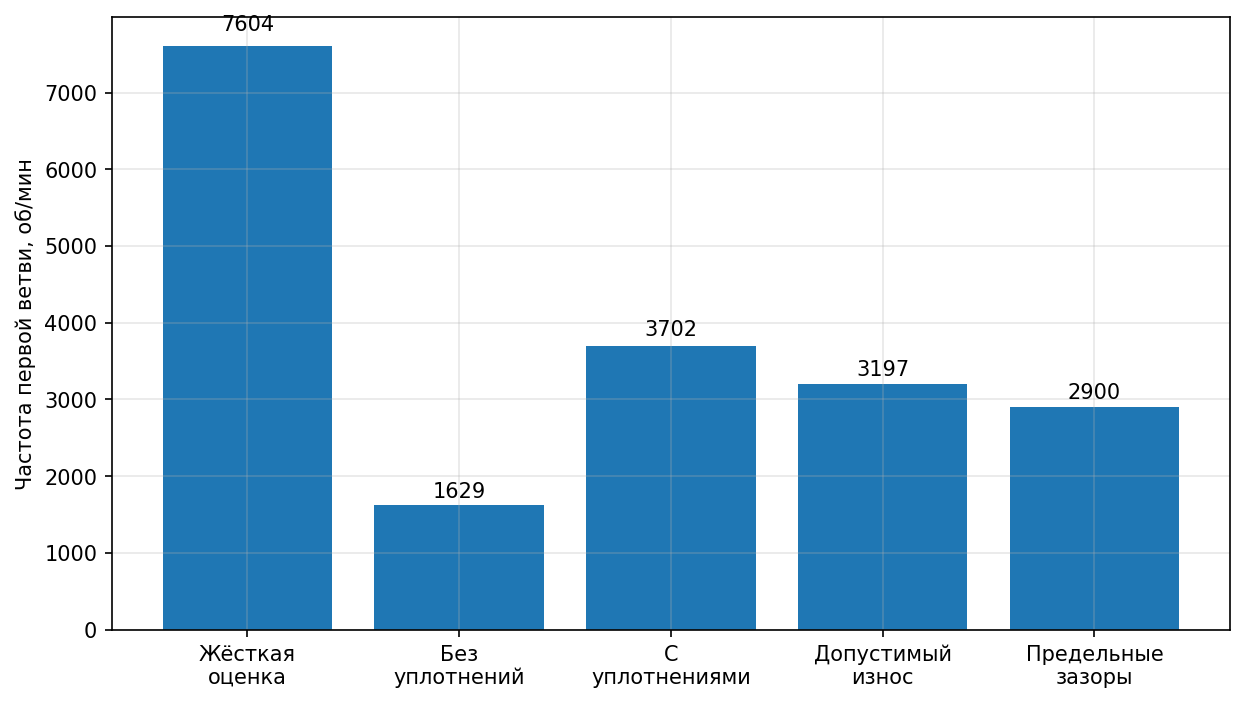
\includegraphics[width=0.85\textwidth]{08_critical_speed_comparison_seals.png}
\caption{Сравнение первой частотной ветви для расчётных вариантов}
\label{fig:critical_comparison}
\end{figure}

Суммарная жёсткость шестнадцати щелевых уплотнений ступеней равна $17$ МН/м, а жёсткость щелевого уплотнения разгрузочного устройства -- $17{,}1$ МН/м. Эти значения меньше жёсткости концевых подшипников, однако их влияние существенно из-за распределения вдоль пакета ступеней. Сопоставление вкладов показано на рисунке \ref{fig:seal_contrib}.

\begin{figure}[H]
\centering

\includegraphics[width=0.85\textwidth]{15_seal_stiffness_contributions.png}
\caption{Сопоставление средней прямой жёсткости опор и щелевых уплотнений}
\label{fig:seal_contrib}
\end{figure}



\subsection{Расчёт орбит}

Для нового ротора при классе G6,3 с номинальной гидравлической радиальной силой полуоси орбиты центрального сечения равны $51{,}6$ и $26{,}95$ мкм. В варианте допустимого эксплуатационного износа при том же классе балансировки, повышенной гидравлической силе и увеличенных зазорах полуоси составляют $252{,}2$ и $121{,}03$ мкм. В предельно допустимом варианте G16 с увеличенными зазорами полуоси возрастают до $488{,}38$ и $285{,}49$ мкм. Амплитуды синхронных сил в этих вариантах составляют соответственно $|F_x|=548$ Н и $|F_y|=289{,}6$ Н, $|F_x|=1064{,}8$ Н и $|F_y|=548$ Н, $|F_x|=1112{,}8$ Н и $|F_y|=595{,}9$ Н.

\begin{figure}[H]
\centering
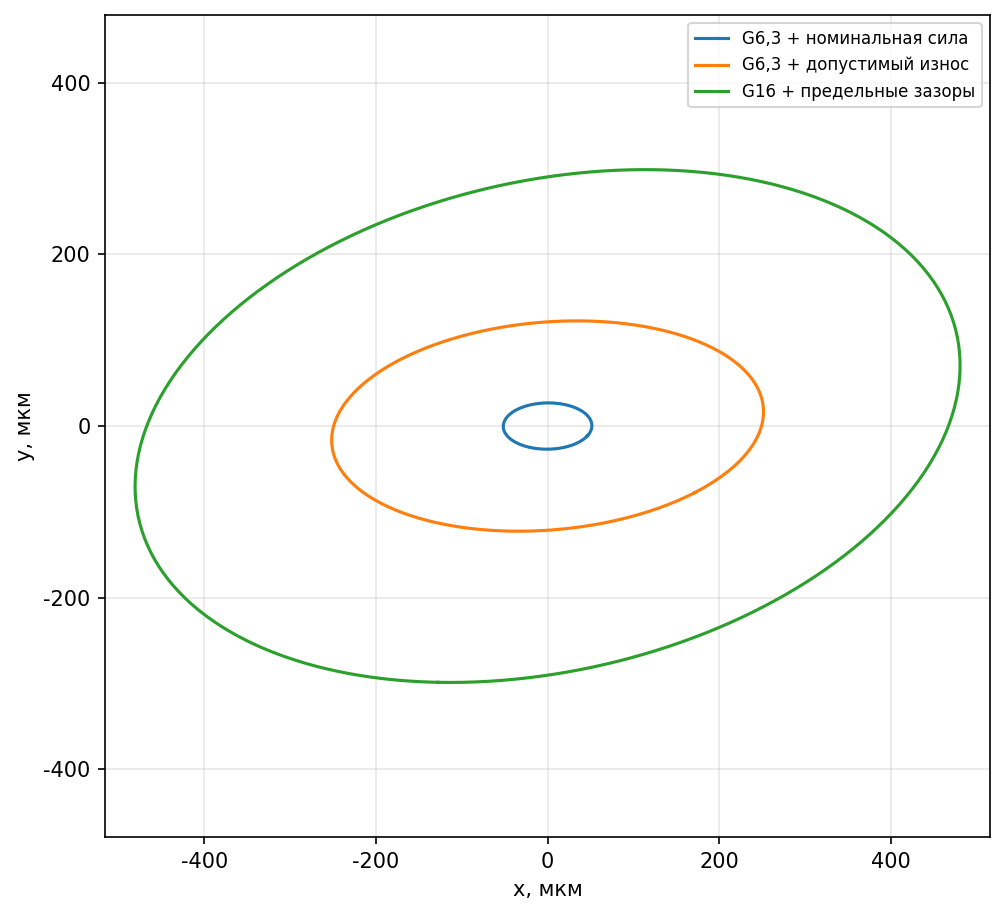
\includegraphics[width=0.75\textwidth]{09_orbits_comparison_seals.png}
\caption{Орбиты центрального сечения при разных эксплуатационных нагрузках}
\label{fig:orbits_center}
\end{figure}

В опорных сечениях влияние матрицы опоры выражено сильнее. На рисунке \ref{fig:support_orbits} показан предельно допустимый вариант G16 с повышенной гидравлической силой и увеличенными зазорами. В левой опоре полуоси составили $64{,}05$ и $5{,}46$ мкм, в правой -- $13{,}41$ и $1{,}48$ мкм. Максимальное отношение полуосей равно $11{,}74$, что указывает на высокую степень эллиптичности орбиты.

\begin{figure}[H]
\centering

\includegraphics[width=0.75\textwidth]{16_support_orbits_full_matrix.png}
\caption{Орбиты в опорных сечениях для предельно допустимого варианта G16}
\label{fig:support_orbits}
\end{figure}

Полученные орбиты подтверждают, что движение в плоскостях $x$ и $y$ не является дублированием одной балочной модели. Эллиптичность связана с различием прямых коэффициентов $K_{xx}$, $K_{yy}$, наличием перекрёстных компонентов матрицы опоры и неравными проекциями эксплуатационной силы.

\subsection{Расчёт перекоса шейки}

По гармонической реакции ротора определены углы поворота опорных сечений. Максимальный угол перекоса шейки закономерно возрастает с увеличением износа: от $0{,}098$ мрад для нового ротора (G6,3, номинальная гидравлическая сила) до $0{,}45$ мрад при допустимом эксплуатационном износе (G6,3, нерасчётный режим, увеличенные зазоры) и $0{,}84$ мрад в предельно допустимом варианте G16. Соответственно минимальный краевой зазор в наиболее нагруженной стороне вкладыша снижается с $32{,}98$ до $25{,}93$ и $18{,}14$ мкм. Сводка по трём сценариям приведена в таблице \ref{tab:misalignment_scenarios}.

\begin{table}[H]
\centering
\caption{Перекос шейки в подшипнике по эксплуатационным сценариям}
\label{tab:misalignment_scenarios}
{\small\setstretch{1.0}
\begin{tabularx}{\textwidth}{>{\raggedright\arraybackslash}X cc}
\toprule
\multicolumn{1}{c}{\textbf{Сценарий}} & \textbf{$\theta_{\max}$, мрад} & \textbf{$h_{min,edge}$, мкм} \\
\midrule
G6,3, номинальный режим & 0{,}098 & 32{,}98 \\
G6,3, допустимый износ & 0{,}45 & 25{,}93 \\
G16, предельные зазоры & 0{,}84 & 18{,}14 \\
\bottomrule
\end{tabularx}}
\end{table}

На рисунке \ref{fig:mis_clearance} показано изменение минимального зазора вдоль длины вкладыша. При $\varepsilon=0{,}347$ зазор без перекоса составляет около $34{,}9$ мкм. Для предельно допустимого варианта минимальный краевой зазор равен $18{,}14$ мкм. Запас по зазору сохраняется, однако влияние перекоса становится заметным.

\begin{figure}[H]
\centering

\includegraphics[width=0.90\textwidth]{12_misalignment_clearance.png}
\caption{Влияние перекоса шейки на минимальный зазор вдоль вкладыша}
\label{fig:mis_clearance}
\end{figure}

На рисунке \ref{fig:mis_pressure} приведено распределение давления вдоль вкладыша в зоне максимального давления. В предельно допустимом варианте максимальное давление увеличивается с $0{,}685$ до $0{,}897$ МПа, то есть на $31\%$. Для выбранного режима это не приводит к потере работоспособности подшипника, но показывает направление влияния перекоса.

\begin{figure}[H]
\centering

\includegraphics[width=0.90\textwidth]{13_misalignment_pressure_axial.png}
\caption{Распределение давления вдоль вкладыша без перекоса и с перекосом}
\label{fig:mis_pressure}
\end{figure}

\subsection{Параметрические исследования}

На рисунке \ref{fig:sweep_eccentricity} показано влияние эксцентриситета на первую частотную ветвь. Увеличение эксцентриситета повышает жёсткость масляной плёнки и заметно увеличивает критическую скорость жёсткой оценки. Для упругой модели первая частотная ветвь практически не меняется: при изменении эксцентриситета от $0{,}2$ до $0{,}8$ она находится в узком диапазоне $1623$--$1634$ об/мин. Это связано с тем, что для длинного многоступенчатого ротора первая критическая скорость определяется преимущественно изгибной жёсткостью вала, а вклад опор является вторичным. Следовательно, расчёт без учёта упругости вала существенно завышает критическую скорость.

\begin{figure}[H]
\centering

\includegraphics[width=0.90\textwidth]{10_sweep_eccentricity.png}
\caption{Влияние эксцентриситета на первую частотную ветвь}
\label{fig:sweep_eccentricity}
\end{figure}

На рисунке \ref{fig:sweep_span} приведено влияние расстояния между опорами. При увеличении пролёта первая частотная ветвь упругой модели снижается, что соответствует росту изгибной податливости вала.

\begin{figure}[H]
\centering

\includegraphics[width=0.90\textwidth]{11_sweep_span.png}
\caption{Влияние расстояния между опорами на первую частотную ветвь}
\label{fig:sweep_span}
\end{figure}

На рисунке \ref{fig:sensitivity} показан анализ чувствительности модели к коэффициенту Ломакина $\lambda_L$ в диапазоне $\pm30\%$ от номинального значения. При изменении $\lambda_L$ от $0{,}385$ до $0{,}715$ первая частотная ветвь меняется от $3258{,}1$ до $4094{,}1$ об/мин, что соответствует отклонению от $-12$ до $+10{,}6\%$. Умеренный характер изменения показывает устойчивость результата к неопределённости коэффициента щелевого уплотнения.

\begin{figure}[H]
\centering

\includegraphics[width=0.90\textwidth]{14_sensitivity_lomakin_lambda.png}
\caption{Анализ чувствительности первой частотной ветви}
\label{fig:sensitivity}
\end{figure}

Сопоставление параметрических исследований показывает, что наибольшее влияние на первую критическую скорость оказывают параметры щелевых уплотнений. Изменение коэффициента Ломакина $\lambda_L$ на $\pm30\%$ смещает первую частотную ветвь на $-12\ldots+10{,}6\%$, тогда как изменение эксцентриситета подшипника в диапазоне $0{,}2$--$0{,}8$ меняет её менее чем на $1\%$. Таким образом, наиболее критичным параметром для динамических характеристик ротора является жёсткость щелевых уплотнений, определяемая коэффициентом Ломакина и радиальным зазором уплотнения, тогда как эксцентриситет и параметры подшипника влияют на первую критическую скорость существенно слабее.


\subsection{Анализ устойчивости и нормативная оценка}

Проверка устойчивости выполнена по комплексным собственным значениям системы первого порядка. В таблице \ref{tab:stability_summary} приведены низшие собственные ветви для трёх эксплуатационных сценариев. Для нового ротора и варианта допустимого износа действительные части первых трёх ветвей отрицательны, поэтому свободные колебания в рабочем диапазоне затухают. Для предельно допустимого варианта G16 третья ветвь имеет $\operatorname{Re}(s_3)=6{,}91$ c$^{-1}$ и отрицательный логарифмический декремент $\delta_3=-0{,}053$, что указывает на потерю запаса устойчивости в расчётной низкочастотной области.

\begin{table}[H]
\centering
\caption{Оценка устойчивости по собственным значениям}
\label{tab:stability_summary}
{\small\setstretch{1.0}
\begin{tabularx}{\textwidth}{>{\raggedright\arraybackslash}X cccc >{\centering\arraybackslash}X}
\toprule
\multicolumn{1}{c}{\textbf{Сценарий}} & \textbf{$n_1$, об/мин} & \textbf{$\operatorname{Re}(s_1)$, c$^{-1}$} & \textbf{$\delta_1$} & \textbf{$\min\delta_{1..3}$} & \textbf{Вывод} \\
\midrule
G6,3, номинальный режим & 3701{,}8 & -46{,}7 & 0{,}757 & 0{,}504 & устойчив, запас по декременту достаточный \\
G6,3, допустимый износ & 3197{,}3 & -34{,}01 & 0{,}638 & 0{,}138 & устойчив, запас по декременту близок к нижней границе \\
G16, предельные зазоры & 2900 & -19{,}35 & 0{,}4 & -0{,}053 & динамический запас потерян по третьей ветви \\
\bottomrule
\end{tabularx}}
\end{table}

На рисунке \ref{fig:log_decrement} показано изменение логарифмического декремента. Первая ветвь остаётся затухающей во всех вариантах, однако минимум по первым трём ветвям снижается от $0{,}504$ в номинальном режиме до отрицательного значения в предельном состоянии. В качестве практического критерия принято условие $\delta\geq0{,}1$, применяемое в ротородинамических проверках по API 684 [12].

\begin{figure}[H]
\centering

\includegraphics[width=0.88\textwidth]{17_log_decrement_stability.png}
\caption{Логарифмический декремент затухания для эксплуатационных сценариев}
\label{fig:log_decrement}
\end{figure}

Для практической интерпретации результаты сопоставлены с нормативными критериями. Для центробежных насосов по API 610 / ISO 13709 рабочая частота должна быть удалена от критических скоростей не менее чем на $15$--$20\%$ [10]. Вибрационная оценка выполнена по ГОСТ Р ИСО 20816 и ISO 20816 для среднеквадратичной виброскорости в опорных сечениях: зоны A/B/C/D используются как укрупнённая шкала состояния машины [11]. Так как расчётная орбита является перемещением вала, виброскорость определялась по максимальной полуоси орбиты в опорном сечении:
\begin{equation}
    v_{\text{rms}}=\frac{a\Omega}{\sqrt{2}},
    \label{eq:rms_velocity_from_orbit}
\end{equation}
\begin{conditions}
$a$ -- большая полуось орбиты, м.
\end{conditions}

Для шкалы зон приняты границы: A -- до $2{,}3$ мм/с, B -- до $4{,}5$ мм/с, C -- до $7{,}1$ мм/с, D -- свыше $7{,}1$ мм/с.

\begin{table}[H]
\centering
\caption{Сравнение эксплуатационных сценариев с нормативными критериями}
\label{tab:normative_summary}
{\small\setstretch{1.0}
\begin{tabularx}{\textwidth}{>{\raggedright\arraybackslash}X cccc >{\centering\arraybackslash}X}
\toprule
\multicolumn{1}{c}{\textbf{Сценарий}} & \textbf{Запас до $n_1$, \%} & \textbf{$a_{\text{оп}}$, мкм} & \textbf{$v_{\text{rms}}$, мм/с} & \textbf{Зона} & \textbf{Практический вывод} \\
\midrule
G6,3, номинальный режим & 25{,}5 & 2{,}14 & 0{,}47 & A & запас по критической скорости и вибрации достаточен \\
G6,3, допустимый износ & 8{,}4 & 26{,}32 & 5{,}75 & C & необходим контроль зазоров и вибрации, длительная работа нежелательна \\
G16, предельные зазоры & 1{,}7 & 64{,}05 & 13{,}99 & D & состояние близко к резонансу и требует вывода в ремонт \\
\bottomrule
\end{tabularx}}
\end{table}

Из таблицы \ref{tab:normative_summary} следует, что новый ротор имеет достаточный частотный запас: первая ветвь находится на $25{,}5\%$ выше рабочей частоты $2950$ об/мин. При допустимом износе первая ветвь снижается до $3197{,}3$ об/мин, запас уменьшается до $8{,}4\%$, поэтому эксплуатация требует контроля вибрации и зазоров. В предельном варианте G16 первая ветвь $2900$ об/мин находится практически на рабочей частоте; одновременно виброскорость попадает в зону D, а третья собственная ветвь имеет отрицательный декремент. Практически это означает необходимость балансировки ротора, контроля щелевых уплотнений и восстановления зазоров подшипников при ремонте.

\subsection{Сравнение расчётных вариантов}

Сравнение вариантов показывает, что динамические характеристики ротора существенно зависят от состояния зазоров и уровня остаточного дисбаланса. Номинальный вариант удовлетворяет критерию удаления от первой критической скорости и имеет положительный логарифмический декремент. При допустимом износе устойчивость первых ветвей сохраняется, однако запас до первой критической скорости становится недостаточным. Предельный вариант G16 с увеличенными зазорами оказывается близким к рабочей скорости и одновременно теряет запас устойчивости по третьей ветви. Учёт гидравлической радиальной силы потока и допустимого износа приводит к орбитам в диапазоне десятков и сотен микрометров, что соответствует инженерно наблюдаемому уровню смещений секционного насоса.

Результаты также показывают важность использования индивидуальных массовых характеристик рабочих колёс. Суммарная масса колёс ЦНС 105-392 по расчётной схеме составляет $131{,}6$ кг при индивидуальном распределении по ступеням. Индивидуальное распределение масс повышает достоверность матрицы масс и расчёта собственных форм.



\subsection{Выводы по третьей главе}

В третьей главе выполнен численный расчёт динамических характеристик ротора насоса ЦНС 105-392. Массовая схема построена по спецификации сборочного чертежа с индивидуальными массами рабочих колёс. Суммарная масса рабочих колёс составляет $131{,}6$ кг, а полная расчётная масса ротора с валом -- $229{,}03$ кг.

Статическое равновесие ротора дало реакции $W_1=1{,}185$ кН и $W_2=1{,}062$ кН. По зависимости несущей способности масляной плёнки от эксцентриситета получены рабочие положения шейки: $\varepsilon_1=0{,}36$ для левой опоры и $\varepsilon_2=0{,}334$ для правой. Таким образом, эксцентриситет подшипника определяется из расчёта статического равновесия опор.

По модели гладкого подшипника при среднем рабочем эксцентриситете $\varepsilon=0{,}347$ получено максимальное давление $0{,}685$ МПа, несущая сила $1{,}102$ кН и минимальный зазор $34{,}95$ мкм. Для базового режима матрица опоры имеет выраженные перекрёстные компоненты: $K_{xx}=5{,}55\cdot10^7$ Н/м, $K_{yy}=2{,}25\cdot10^7$ Н/м, $K_{xy}=5{,}46\cdot10^7$ Н/м и $K_{yx}=-7{,}36\cdot10^7$ Н/м.

Комплексный расчёт собственных частот показал разделение первой пары на ветви прямой и обратной прецессии. Без щелевых уплотнений первая пара равна $1629{,}3$ и $1634{,}2$ об/мин. При учёте щелевых уплотнений первая пара повышается до $3701{,}8$ и $3705{,}7$ об/мин. Для варианта допустимого износа первая ветвь снижается до $3197{,}3$ об/мин, а для предельно допустимого варианта G16 с увеличенными зазорами -- до $2900$ об/мин, то есть оказывается близкой к рабочей скорости $2950$ об/мин.

Расчёт орбит с эксплуатационными нагрузками дал инженерно значимые амплитуды. Для нового ротора G6,3 с номинальной гидравлической силой полуоси орбиты центрального сечения составляют $51{,}6$ и $26{,}95$ мкм. Для варианта допустимого износа полуоси возрастают до $252{,}2$ и $121{,}03$ мкм, а для предельно допустимого варианта G16 -- до $488{,}38$ и $285{,}49$ мкм. В опорных сечениях орбиты имеют эллиптическую форму с отношением полуосей до $11{,}74$, что отражает анизотропию и перекрёстные коэффициенты подшипника.

Анализ устойчивости показал, что в номинальном режиме первая ветвь имеет $\operatorname{Re}(s_1)=-46{,}7$ c$^{-1}$ и $\delta_1=0{,}757$, а минимальный декремент первых трёх ветвей равен $0{,}504$. При допустимом износе минимальный декремент снижается до $0{,}138$, но остаётся выше ориентировочного критерия $0{,}1$. В предельном варианте G16 третья ветвь имеет $\operatorname{Re}(s_3)=6{,}91$ c$^{-1}$ и $\delta_3=-0{,}053$, поэтому динамический запас считается потерянным. Нормативное сопоставление показало: новый ротор имеет запас по критической скорости $25{,}5\%$ и зону вибрации A в опорном сечении; при допустимом износе запас снижается до $8{,}4\%$ и виброскорость переходит в зону C; в предельном состоянии запас составляет только $1{,}7\%$, а виброскорость соответствует зоне D.

Гидравлическая радиальная сила, рассчитанная по реальным параметрам колеса $D_2=0{,}3$ м и $B_2=0{,}0224$ м, составляет $516{,}8$ Н на номинальном режиме и $1033{,}7$ Н на нерасчётном режиме. Допустимый дисбаланс по чертежу $D_b=250$ г$\cdot$мм даёт силу $23{,}86$ Н, что совпадает по порядку с оценкой по классу G6,3. Анализ чувствительности к коэффициенту Ломакина показал изменение первой частотной ветви от $-12$ до $+10{,}6\%$ при изменении $\lambda_L$ на $\pm30\%$, поэтому результат устойчив к разумной неопределённости параметров щелевых уплотнений.


% Заключение
\newpage
\phantomsection
\addcontentsline{toc}{section}{Заключение}
\section*{ЗАКЛЮЧЕНИЕ}

% TODO: написать заключение (основные результаты и выводы по работе).
Текст заключения будет добавлен.


% Список использованных источников
\newpage
\phantomsection
\addcontentsline{toc}{section}{Список использованных источников}
\section*{СПИСОК ИСПОЛЬЗОВАННЫХ ИСТОЧНИКОВ}
\begin{enumerate}
    \item Ломакин А. А. Центробежные и осевые насосы. 2-е изд., перераб. и доп. Москва; Ленинград: Машиностроение, 1966. 364 с.
    \item Михайлов А. К., Малюшенко В. В. Лопастные насосы. Теория, расчёт и конструирование. Москва: Машиностроение, 1977. 288 с.
    \item Ломакин А. А. Расчёт критического числа оборотов и условий обеспечения динамической устойчивости роторов гидравлических машин высокого давления с учётом сил в уплотнениях // Энергомашиностроение. 1958. № 4. С. 1-8.
    \item Childs D. W. Turbomachinery Rotordynamics: Phenomena, Modeling, and Analysis. New York: Wiley, 1993.
    \item Lund J. W. Review of the Concept of Dynamic Coefficients for Fluid Film Journal Bearings // ASME Journal of Tribology. 1987. Vol. 109, no. 1. P. 37-41.
    \item Никитин Г. А. Щелевые и лабиринтные уплотнения гидроагрегатов. Москва: Машиностроение, 1982.
    \item Уплотнения и уплотнительная техника: справочник / под общ. ред. А. И. Голубева, Л. А. Кондакова. Москва: Машиностроение, 1986.
    \item Марцинковский В. А. Бесконтактные уплотнения роторных машин. Москва: Машиностроение, 1980.
    \item Марцинковский В. А. Щелевые уплотнения: теория и практика. Сумы: Изд-во СумГУ, 2005.
    \item Black H. F., Jenssen D. N. Dynamic hybrid bearing characteristics of annular controlled leakage seals // Proceedings of the Institution of Mechanical Engineers. 1969. Vol. 184. P. 92-100.
    \item Hirs G. G. A bulk-flow theory for turbulence in lubricant films // Journal of Lubrication Technology. 1973. Vol. 95, no. 2. P. 137-146.
    \item San Andrés L. Analysis of turbulent annular seals with fluid inertia effects // ASME Journal of Tribology. 1991. Vol. 113. P. 302-309.
    \item ГОСТ ИСО 1940-1-2007. Вибрация. Требования к качеству балансировки жёстких роторов. Часть 1. Определение допустимого остаточного дисбаланса. Москва: Стандартинформ, 2008.
    \item Xiong G., Zhang J., Mao Z., Wang Z., Wang H., Lian S., Jiang Z. Dynamic misalignment effects on performance of dynamically loaded journal bearings // International Journal of Mechanical Sciences. 2024. Vol. 264. Article 108839.
    \item Xie Z., Jiao J., Zhao B., Zhang J., Xu F. Theoretical and experimental research on the effect of bi-directional misalignment on the static and dynamic characteristics of a novel bearing // Mechanical Systems and Signal Processing. 2024. Vol. 208. Article 111041.
    \item Кельзон А. С., Журавлёв Ю. Н., Январёв Н. В. Расчёт и конструирование роторных машин. Ленинград: Машиностроение, 1977. 288 с.
    \item Тимошенко С. П., Янг Д. Х., Уивер У. Колебания в инженерном деле / пер. с англ. под ред. Э. И. Григолюка. Москва: Машиностроение, 1985. 472 с.
    \item Vance J. M., Zeidan F. Y., Murphy B. G. Machinery Vibration and Rotordynamics. Hoboken: John Wiley \& Sons, 2010.
    \item Genta G. Dynamics of Rotating Systems. New York: Springer, 2005. 658 p.
    \item Adams M. L. Rotating Machinery Vibration: From Analysis to Troubleshooting. 2nd ed. Boca Raton: CRC Press, 2010.
    \item API Standard 610. Centrifugal Pumps for Petroleum, Petrochemical and Natural Gas Industries. 12th ed. Washington: American Petroleum Institute, 2021; ISO 13709:2009. Centrifugal pumps for petroleum, petrochemical and natural gas industries. Geneva: ISO, 2009.
    \item ГОСТ Р ИСО 20816-3-2023. Вибрация. Измерение и оценка вибрации машин. Часть 3. Машины промышленного назначения номинальной мощностью более 15 кВт и номинальными скоростями от 120 об/мин до 30000 об/мин. Москва: Стандартинформ, 2023.
    \item API Recommended Practice 684. API Standard Paragraphs Rotordynamic Tutorial: Lateral Critical Speeds, Unbalance Response, Stability, Train Torsionals, and Rotor Balancing. 4th ed. Washington: American Petroleum Institute, 2014. Reaffirmed 2022.
    \item ГОСТ 801-78. Сталь подшипниковая. Технические условия. Москва: Издательство стандартов, 1978.
    \item Mota J. A., Maldonado D. J. G., Valério J. V., Ritto T. G. Complete modeling of hydrodynamic bearings with a boundary parameterization approach // Mechanism and Machine Theory. 2021. Vol. 162. Article 104350.
    \item Степанов А. И. Центробежные и осевые насосы. Москва: Машгиз, 1960.
    \item Gu C., Meng X., Wang S., Ding X. Modeling a hydrodynamic bearing with provision for misalignments and textures // Journal of Tribology. 2020. Vol. 142. Article 041801.
    \item ТУ 3631-003-00217389-96. Насосы центробежные секционные типа ЦНС. Технические условия.
    \item Колесо рабочее 1 ступени ЦНС 90.00.00.012. Чертёж детали, УГНТУ МП-98-02.
    \item ГОСТ 31381-2009. Насосы динамические. Методы испытаний. Москва: Стандартинформ, 2010.
\end{enumerate}


\end{document}
